\chapter{System design} \label{des}
\section{Introduction}
This chapter defines aim of the project and specifies potential users of the application. Secondly, it breaks down requirements that were set for this project into separate sections - functional, non-functional, hardware, software and quality -  where they are described in detail. Next, the project of the system is presented by UML and classes diagrams. Finally, the most important libraries used for document classification framework are defined.

\section{Aim of the project}
Main aim of this project is to develop platform for automated text document classification. Proposed solution will be capable of classificating text documents with a focus on parallel execution of algorithms. Classificator will implement a dual-layer model. In first layer a k-Nearest-Neighbors [\ref{soa-knn}] algorithm will be used for a general decision narrowing the set of possible membership classes. More detailed and precise classification decision will be made by second layer with Support Vector Machine [\ref{soa-svm}] algorithm.

The application will be created with the intent of providing a complete set of tools for text document classification and documenting usability of various machine learning algorithms. This includes:
\begin{itemize}
	\item \textbf{feature extraction} - creating feature vectors for text documents, methods for reducing vectors dimensionality,
	\item \textbf{clusterization} - finding groups of similar documents that would define clusters,
	\item \textbf{classification} - defining position of new documents in cluster space and finding its best matching group membership,
	\item \textbf{algorithms performance tests and results} - all algorithms will be tested with various parameters and the results will be described.
\end{itemize}

Final solution should also indicate how complex the computation part is and how crucial it is to design a system that supports parallel tasks execution, distributes workloads in efficient manner between available worker processes and makes a proper use of all available resources.

The project may become a useful tool not only as a base framework for data scientists, but also for writers whom it should aid assigning a proper label to the document.

\section{Potential users} \label{design-users}
The application will be dedicated mainly to data scientists, for whom it could act as a base natural language processing and classification framework. Application's design will make it possible to add new modules and test the flow in high performance parallel environment.

On the other hand users like article writers and administrators of knowledge bases will also be able to use this tool. For writers it might serve as an advisor which will help to mark document with proper labels, removing the burden of having to know the context of other documents already in the database. For knowledge base administrators this framework might be convenient way keeping the database and documents grouped in a consistent way.

\section{System requirements}
In this section requirements for this project are defined. It starts with placing application in today's business context, where examples of possible adaptations are described, and the prospect of tomorrow, which outlines the possible ways of evolution. Next, the non-functional and functional requirements are described along with the example of use cases. Next, it describes software and hardware requirements, outlining minimal configuration that must be met and recommending hardware parameters that would help increase overall applications performance. Finally, architecture and design are described in detail and illustrated with class, sequence and flow diagrams.

\subsection{General requirements}
	
	\begin{enumerate}
	
	\item \textbf{Business context}
	Application will be implemented with portability in mind. Everone will be able to use it by downloading and running localy, either on commodity hardware or server-grade workstations with multiple processors. This project will make management of knowledge databases more attractive in the context of:
	
	\begin{enumerate}
		\item keeping database clean and well organized by sorting documents into seperate categories
		\item providing means of assigning label to new document without forcing user to have knowledge of all documents context
	\end{enumerate}
	
	Furthermore application will be available freely online, so everyone will be able to use it. Furthermore, because of releasing it under GPLv2 license, one will be able to adapt framework to ever changing goals by being able to change code base, all algorithms and adding new modules. This release approach will make the application more available to all potential users, thus helping to increase its user-base.  
	
	\item \textbf{Prospectiveness}
	
	Application will be designed with object oriented principles, enabling it being part of a larger system by exposing different interfaces. In the future application could be adapted to users needs and play a part in bigger system. As the implementation itself is modular, it is possible to add, remove or rearrenge logic blocks inside of application. This indicates the prospectiveness of proposed system, its agile approach and possibility of including it as a part of another platform.
	
	\end{enumerate}

\subsection{Functional requirements}
TODO
Diagram presented in the figure \ref{functional} shows general functional requirements available in the application. The aim of the diagram is to describe possible interactions between actors and functions offered by the application. Each oval shows a single use case within which different flows called scenarios may occur. Every use case characterizes possible system functionalities and defines steps that lead to the effect observable by the actor. A dependency marked as \textbf{extend} describes some additional behavior, which in some cases may be included into the base use case. 
The base use case is the one which is pointed by the arrowhead of the connection. The extend use case continues the behavior of the base use case by inserting additional actions into the base sequence when the appropriate extension point is reached in the base use case and the extension condition is filled. An \textbf{include} dependency is a relationship which describes the inclusion of another use case responsible for different behavior. The including dependency is the one pointed by the arrowhead of the connection.


To present more detailed interactions, use cases from following categories were extended and shown on separate diagrams.
\begin{figure}[H]
	\begin{center}
		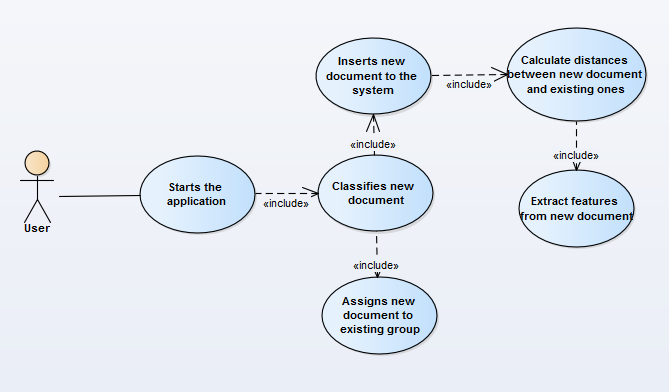
\includegraphics[width=1.0\linewidth]{images/diagrams/use-case/use-case-11.PNG}
		\caption{Example of ROC curve, source \cite{roc-curve}}
		\label{design-use-case-1}
	\end{center}
\end{figure}

\begin{figure}[H]
	\begin{center}
		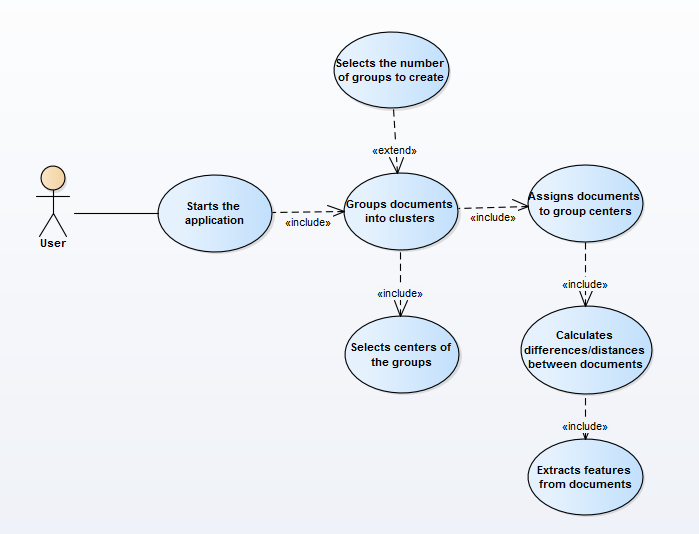
\includegraphics[width=1.0\linewidth]{images/diagrams/use-case/use-case-22.PNG}
		\caption{Example of ROC curve, source \cite{roc-curve}}
		\label{design-use-case-2}
	\end{center}
\end{figure}
 
Descriptions of all of the use cases including their initial, alternative and results were collected in the table \ref{tab:tableusecase}.
\vspace{5em}

< tutaj tabelka>
    
\subsection{Non functional requirements}
TODO
\textbf{Quality requirements}


\textbf{Ergonomy}
\label{interfaceerg}


\textbf{Restrictive requirements}

A user of the application, will have to have basic skills of 


In order to use the application the following software and hardware requirements will have to be filled.

\subsection{Hardware and software requirements}
In this section software and hardware requirements are described.

\subsubsection{Hardware requirements}
This application will be tested on various hardware configuration to prove that it can work reliable on even older machines. Although the following configuration is not a server-grade hardware, it may allow to execute flow of the application without running out of available resources in most of the presented test cases. It will be considered as a recommended minimal configuration.
\begin{itemize}
	\item Processor - at least a quad-core processor is recommended. Usage of technologies like Intel's HyperThreading is not advised and the number of spawned child processes should not exceed the number of physical cores. Application will rely heavily on reads and writes to shared memory, thus limiting use of virtual cores (\cite{performance_ht}). Processor used during tests will be Intel i7 with 4 physical cores and 8 logical processors.
	\item System memory - probably will have the greatest impact on performance of the application. The more memory, the less caching mechanisms will be used. Caching uses hard drives as a backend for storing processed documents, which greatly affects overall performance and execution time. Machine with 16 GB DDR3 memory will be used during tests.
	\item Hard drives - speed of reads and writes to hard drives is a crucial factor during startup of application and in case of using cache. SSD drive should be considered in place of standard hard drive due to higher speeds of reads and writes and O(1) latency of access \cite{performance_hdd_ssd}. A SSD drive connected to PCI-e slot will be used during tests.
\end{itemize}


\subsubsection{Software requirements}
There are no specified requirements about the operating system installed on the device. Application should run on every modern operating system, being it either Linux, OS X or Windows. Tests will be run on both Linux and OS X machines, however the Windows environment will be never fully tested and thus is not recommended for running the application.

Taking software requirements into consideration, a Python interpreter will have to be installed on a machine along with a set of libraries. Python is an interpreted language that provides good performance, scalability features and possibility of adapting software on-the-fly without a need to recompile the code. All required libraries are listed in both section \ref{design-libraries} and in source code in \textit{source/requirements3.txt} file.
 
 
\section{Project of a system} \label{project}
TODO
This section provides the project of the described solution for......

 The project was presented by the diagrams employed in UML (Unified Modeling Language), a standard notation for the modeling of real-world objects and systems. 
 
\subsection{Activity diagram of the performing test flow}
TODO
The activity diagram shows the logic of workflows of step-wise actions. Rectangles with rounded corners present sequences of activities. A rhombus represents a decision after which it is possible to choose one of the alternatives. A diagram in the figure \ref{activity} shows a sequence of actions needed to ......

........ is a starting point, ....... is a final point. 


\subsection{Sequence diagram of processing frames}
TODO



\subsection{Diagram of classes}
TODO
A diagram of classes (figure \ref{classes})is one of the most popular UML diagrams. Rectangles show classes, their attributes and methods. Association connections were used to present relations between entities. Classes communicates with each other by sending messages (by association connections) and as a result they are able to fill tasks presented on the dynamic diagrams, for example use case model \ref{tab:tableusecase}.

 
  

\subsection{Architecture}
TODO
The whole application will be based on ....... model. It is a distributed application structure that partitions tasks between the ..........


The main idea of this model is presented in the figure \ref{client}.
 
 
 
 
\subsection{Libraries} \label{design-libraries}
This project is designed to be portable across different platforms and to have minimal dependencies. It will use Python platform and libraries that are freely available via pip, the Python package installer.

Platform dependencies that will have to be installed by user:
\begin{itemize}
	\item \textbf{Python 3.5.1} - the Python language interpreter.
	\item\textbf{pip 8.1.2} - Python package installer.
\end{itemize}

Libraries that are available in default Python 3.5 installation and thus will not require additional steps to install:
\begin{itemize}
	\item \textbf{multiprocessing} - will be used for parallelisation mechanisms. Contains basic shared memory data structures and allows for usage of processes. Processes will be chosen over threads because they are not blocked by Python's Global Interpreter Lock (GIL) and allow to execute tasks in parallel not only locally, but also over network.
	\item \textbf{xml.sax} - will be used to access XML files using streams. Allows to open files that are too big to fit in memory.
\end{itemize}

External Python libraries that can be installed using pip:
\begin{itemize}
	\item \textbf{nltk 3.2.1} - Natural Language ToolKit - is used for word stemming thanks to build-in WordNet
	\item \textbf{SQLAlchemy 1.0.14} - library that will be used for database queries. It is optional, as this project uses database as a cache only when requested by user. By default a sqlite database will be used as a backend because it does not have any additional requirements and is very portable. While its performance may suffer as it does not offer any database management system, it is not the problem in project's implementation.
\end{itemize}


\subsection{Application release}
Presented solution will be developed as an open-source application under GPLv2 license and will be freely available to everyone for using, testing or modifying purposes. Its both source code and documentation will be available online at \href{https://github.com/macsz/parallel-wiki-classifier}{git repository\footnote{https://github.com/macsz/parallel-wiki-classifier} hosted on GitHub}.


\section{Conclusion}
TODO
This chapter includes a complete description of the methodology used to prepare analysis of the requirements for the created application. The proposed algorithm takes advantage of the possibilities of new technologies to .......

Moreover the project of the system was also described and presented taking into consideration all of the specified requirements.
